\chapter{Niveau 3 : La Tombe Inférieure}\label{n3}
\section{Structure}
Il y a deux chemins principaux "horizontaux" et trois "verticaux".
Le donjon bifurque et reboucle.

Il est possible de remonter à la surface comme de plonger plus profond.
Ou même de revenir de là où l'on est parti.
Cet étage est indubitablement plus dangereux que les précédents.

La diplomatie et le troc font également leur apparition, de même que les \nameref{monster:n3:errants}.
Vous pouvez explorer les niveaux 1 et 2 à votre rythme, mais passer trop de temps au Niveau 3 revient à prendre des risques inconsidérés.

La conclusion de cet étage est ouverte : vous pouvez ajouter du contenu pour étendre ce donjon autant que vous le souhaitez.
Arrivé là, si vous êtes un nouveau MJ ou débutant en jeux OSR, vous devriez être prêt à écrire votre propre donjon.

\section{Zones Thématiques}
\subsection{Les Terriers Gobelins}
Les Gobelins Fongiques sont le miroir des PJ, leur opposé.
Ils se complaisent dans la crasse, revivent sans cesse et commettent toujours les mêmes erreurs.
Ils sont affamés, stupides, superstitieux et meurtriers, mais néanmoins attachants.
Les terriers sont l'irruption d'un barbarisme bruyant et enthousiaste dans la civilisation froide et moribonde.

Décrivez les terriers tant par le bruit que par l'odeur.
Ça pue.
Vous allez puer si vous vous attardez ici, et la Tombe des Rois Serpents n'est pas pourvue de bains.
Des petits yeux de gobelins dans la pénombre.
Des dents cliquetantes et des couteaux aiguisés.

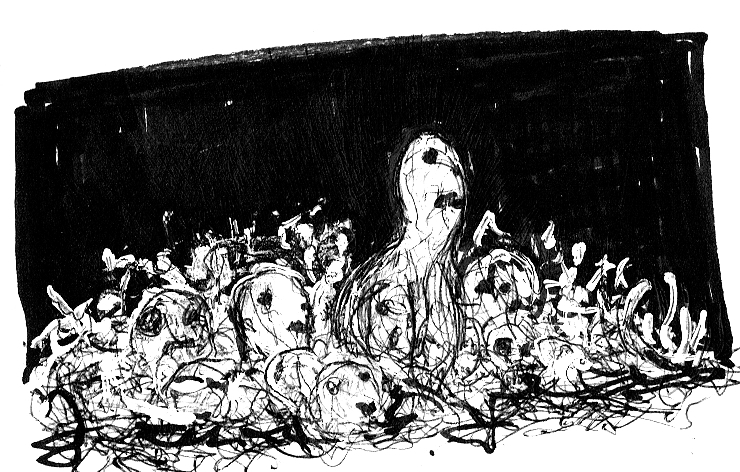
\includegraphics[width=\columnwidth]{pics/goblin_pit.jpg}

\vfill
\pagebreak
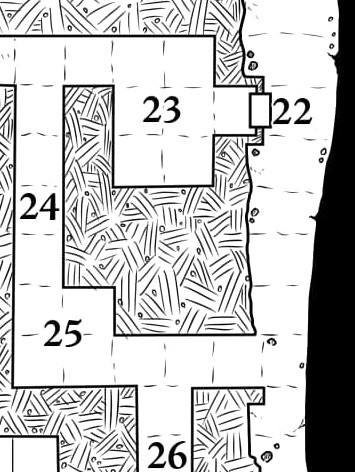
\includegraphics[width=\columnwidth]{pics/map_22-25.jpg}
\subsection{22 : Porte de Pierre}\label{n3:s22}
\begin{itemize}
  \item Enfoncée d’1,50m dans le mur
  \item Maintenue fermée par une lourde barre de pierre côté gouffre. 
  \item En arrivant par l’autre côté, la porte ne peut être ouverte sans être détruite.
  \item \textbf{Piège :}
  \begin{itemize}
    \item Même que \nameref{n1:s5}
    \item Marteau vers l’extérieur :
    \begin{itemize}
      \item 1D6 dommage \textbf{puis :} (sauvegarde contre la mort +2 annule) 
      \item Poussé dans le gouffre (sauvegarde contre la mort annule)
    \end{itemize}
  \end{itemize}
\end{itemize}

\subsection{24 : Couloir}\label{n3:s24}
\begin{itemize}
  \item Couloir de 3m sur 12m, 3m de haut
  \item Sent légèrement l'\textbf{acide}
  \item Bruits de \textbf{claquements humides}.
  \item Descend en pente douce vers le sud.
  \item \textbf{\nameref{monster:n3:squelgel}} au sud attiré par le bruit
\end{itemize}

\subsection{23 : Salle Cérémonielle}\label{n3:s23}
\begin{itemize}
  \item Salle de 6m sur 9m, 3m de haut
  \item Sent les \textbf{champignons séchés} et la \textbf{poussière}.
  \item Bancs au centre
  \item Anciennes tapisseries aux murs
  \item Fontaine asséchée (mur sud) : 
  \begin{itemize}
    \item Résidus d'or (10PO) sur espace plat au milieu
  \end{itemize}
\end{itemize}

Utilisée autrefois par les prêtres hommes-serpents pour se préparer et méditer. 

Les gobelins ont arraché la statue d’or qui ornait la fontaine pour la cacher dans leur salle du trône.

\subsection{25 : Fosse Piégée}\label{n3:s25}
\begin{itemize}
  \item Salle de 6m sur 6m, 3m de haut 
  \item Air \textbf{froid}
  \item Carrelage de dalles : 
  \begin{itemize}
    \item certaines cassées
    \item une manquante
  \end{itemize}
  \item \textbf{Piège :}
  \begin{itemize}
    \item Corniche large de 30 cm le long des murs \textbf{sûre}
    \item Autres carreaux ne sont soutenus que par de fines barres de métal
    \item Pied dans la zone centrale :
    \begin{enumerate}
      \item \textbf{Chute :} 1D6 dégâts (sauvegarde contre la mort annule)
      \item \textbf{Empalé} par les pics au fond : 1D6 dégâts (sauvegarde contre la mort annule)
    \end{enumerate}
  \end{itemize}
\end{itemize}

La fosse contient plusieurs squelettes d’humains normaux, ainsi qu’un anneau d’or valant 20 PO. 

Les gobelins remplacent les dalles chaque jour : ils utilisent le piège pour capturer leurs proies.

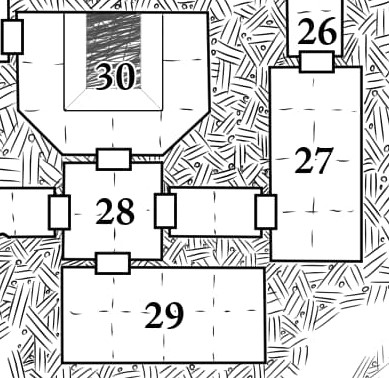
\includegraphics[width=\columnwidth]{pics/map_26-30.jpg}
\subsection{26 : Couloir}\label{n3:s26}
\begin{itemize}
  \item Couloir de 3m sur 6m, 3m de haut
  \item Mène à porte verrouillée :
  \begin{itemize}
    \item \textbf{Serrure aisée :} capacité voleur x2
    \item \textbf{Corrodée :} considérer comme une porte bloquée
  \end{itemize}
\end{itemize}

\subsection{27 : Salle des Esclaves}\label{n3:s27}
\begin{itemize}
  \item Salle de 6m sur 12m, haute de 3m
  \item Air \textbf{chaud et vicié}. 
  \item Taches de sang et roche usée
  \item \textbf{Sifflement} constant au sud-est.
  \item \textbf{Entraves rouillées} au sol.
  \begin{itemize}
    \item Se referment aux jambes si à moins de 30cm
    \item Rouille : Brisées avec test de force
  \end{itemize}
\end{itemize}

\vfill
\pagebreak
\subsection{28 : Dôme}\label{n3:s28}
\begin{itemize}
  \item Salle de 6m sur 6m, haute de 6m
  \item Air \textbf{chaud et vicié}. 
  \item \textbf{Sifflement} constant au nord.
  \item Plafond : \textbf{Dôme},  fresques d’hommes-serpents triomphants
  \item Porte au milieu de chaque mur.
  \item Porte sud verrouillée :
  \begin{itemize}
    \item Clef est au cou du Basilic (p. 14)
    \item Trop épaisse pour être brisée
  \end{itemize}
  \item Porte de pierre brisée à l’est. 
  \item Porte de pierre entrouverte vers le nord.
\end{itemize}

\subsection{29 : Salle du Trésor}\label{n3:s29}
\begin{itemize}
  \item Salle de 12m sur 6m, haute de 6m
  \item Contient tout ce que le MJ jugera bon de mettre au fond d’un donjon. [2000 PO au moins]
\end{itemize}

\subsection{30 : Fosse Sacrificielle}\label{n3:s30}
\begin{itemize}
  \item Salle de 12m sur 9m, haute de 6m
  \item Air vicié,
  \item \textbf{Flamme orangée} au nord, au fond d’une fosse profonde de 5m  aux parois en pente.
  \item Feu est alimenté par du gaz naturel acheminé depuis une antique mine perdue dans les tréfonds
  \item Chemin large de 60 cm borde le trou
  \item \textbf{Os carbonisés} couvrent le fond
  \item \textbf{Coulures d’or} sont visibles autour de la flamme 
  \item \textbf{Pierres précieuses} couvertes de carbone (500 PO en tout) scintillent dans la lueur orangée du feu
  \item Si PJ entrent dans la fosse :
  \begin{itemize}
    \item -1D6 CON (temporaire, sauvegarde poison annule)
    \item 0 CON : inconscient, glisse jusqu'à la flamme :  2d6 dégâts de feu par round
  \end{itemize}
\end{itemize}
